
\section{Multivariate analysis}
\label{sec:mva}

After the traditional cut-based analysis presented in the previous section,
and combining the significance of the different event categories,
we end up with a $S/\sqrt{B}$ value of AAA.
%
Taking into account our more realistic simulation of the QCD background as
compared to previous studies, this is not too bad.
%
However, the attentive reader might have noticed that we have used
relatively 
loose kinematics cuts, for example in the Higgs mass window.
%
The motivation for this is that the $n$-tuples of signal and background
events, after our basic selection, are processed though a multivariate
analysis with the motivation to increase the signal over background
significance.
%
Multivariate techniques are by now a common tool to enhance signal
significance in HEP analysis.

\subsection{MVA strategy}

The classification of events as arising from either signal or
background processess via the use of a multivariate analysis is a common
technique in high energy physics.

In order to investigate the potential efficacy of an MVA in an $HH\to 4b$
measurement, we process the events remaining after the cut-based analysis 
through a standard feed-forward artificial neural network with architecture

\be
\label{eq:nn1}
N_{\mathrm{var}}\times5\times3\times1 \, ,
\ee
where $N_{\mathrm{par}}$ represents the number of input variables for the MVA.
All neural-network layers use a sigmoid activation function, allowing for a probabilistic
interpretation of the neural-network output.

The input variables for the MVA differ between our three categories, based upon
the availability in each analysis of substructure information on fat jets. For all
three analyses, the following common variables are used:

\begin{itemize}
\item The transverse momenta of the leading and subleading Higgs candidates, $p_{T,H_0}$, $p_{T,H_1}$.
\item The transverse momentum of the reconstructed Higgs pair, $p_{T,HH}$
\item The invariant masses of the leading and sub-leading Higgs candidates, $m_{H,1}$, $m_{H,2}$.
\item The invariant mass of the reconstructed Higgs pair, $m_{HH}$.
\item The separation in $R$ of the two Higgs candidates, $\Delta R_{HH}$.
\item The separation in $\phi$ of the two Higgs candidates, $\Delta \phi_{HH}$.
\item The separation in $\eta$ of the two Higgs candidates, $\Delta \eta_{HH}$.
\item The transverse momenta of the leading Higgs candidate subjets, $p_{T,H_{0,0}}$, $p_{T,H_{0,1}}$
\item The transverse momenta of the sub-leading Higgs candidate subjets, $p_{T,H_{1,0}}$, $p_{T,H_{1,1}}$
\end{itemize}

For analyses including the reconstruction of fat jets, the following variables are included for
every fat jet Higgs candidate present in the analysis.

\begin{itemize}
\item The $k_T$ splitting scale of the fat-jet (Reference).
\item The ratio of 2-to-1-Subjettiness $\tau_{2}/\tau_{1}$ of the fat-jet (Reference).
\item The fat-jet energy correlation function double-ratio $C_2$ (Reference).
\item The fat-jet energy correlation function double-ratio $D_2$ (Reference).
\end{itemize}

Therefore there are in total $N_{\mathrm{var}}=13$ variables for the resolved analysis, 17 for the semi-resolved, and 21 for the boosted category.

Given the above set of kinematic variables $\{k\}_i$ associated with the event $i$, and a set of neural network parameters $\{\omega\}$, we interpret the neural network output $y_i$ as the probability that the event $i$ originates from the signal process,
\be y_i = P(y^\prime_i=1|\{k\}_i, \{\omega\} ), \ee
where $y_i^\prime$ represents the true classification of the event $i$, i.e $y^\prime_{\text{signal}} = 1$ and $y^\prime_{\text{background}} = 0$. With this interpretation, our general classification probability including background events is given by
\be
P(y_i^\prime|\{k\}_i, \{\omega\}) = y_i^{y^\prime_i}(1-y_i)^{1-y^\prime_i}.
\ee
 Correspondingly the negative log-liklihood cost function to be used in the neural network training is the cross-entropy error
\be E(\{\omega\}) = -\log\left(\prod_i^{N_{\text{evt}}} P(y_i^\prime|\{k\}_i, \{\omega\})\right) = \sum_i^{N_{\text{evt}}} y^\prime_i\log{y_i} + (1-y^\prime_i)\log{(1-y_i)}. \ee

Using the cross-entropy cost function, the neural networks are trained with a basic genetic algorithm (GA) over 50,000 generations.
(Do we need to specifiy GA params etc?).
\subsection{Enhancing signal discrimination with the MVA}

Now we show the results of the MVA training on the signal and
background samples.
%
First of all in Fig.~\ref{fig:nnresponse} we show
the neural network classification of events is demonstrated for both the resolved and boosted cases.
%
In this figure, we show which is the distribution of the neural network
response, that is, the value of the outer layer in Eq.~(\ref{eq:nn1}),
for signal and background events.
%
For the MVA discrimination to be successful, one needs to find
distinct distributions for the two types of events.
%
As can be seen from  Fig.~\ref{fig:nnresponse}, both
in the boosted and in the resolved cases signal and background
distributions are noticeably different: we can use this property
to introduce the final cut in our analysis, a cut in the value
of the neural network output.

%%%%%%%%%%%%%%%%%%%%%%%%%%%%
\begin{figure}[t]
\begin{center}
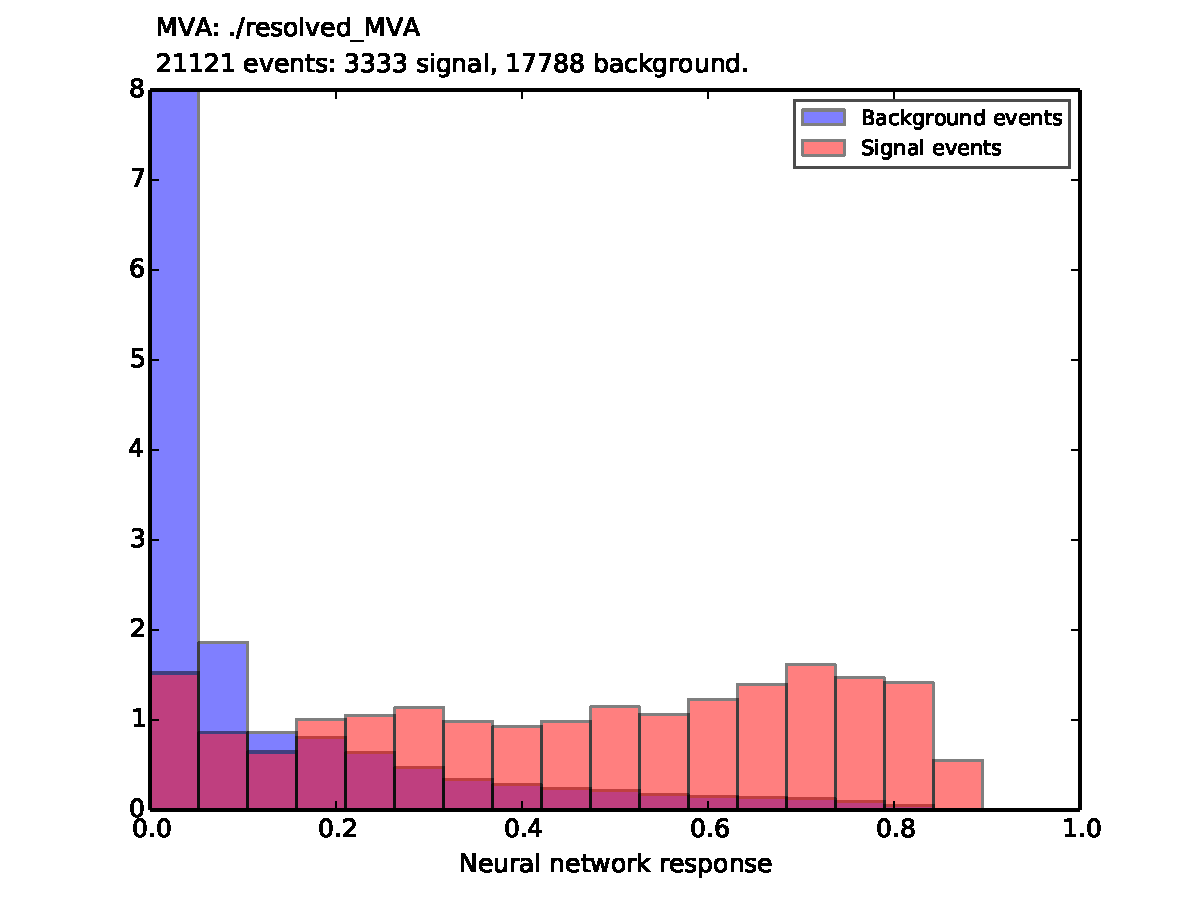
\includegraphics[width=0.48\textwidth]{plots/resolved_MVA_hist.pdf}
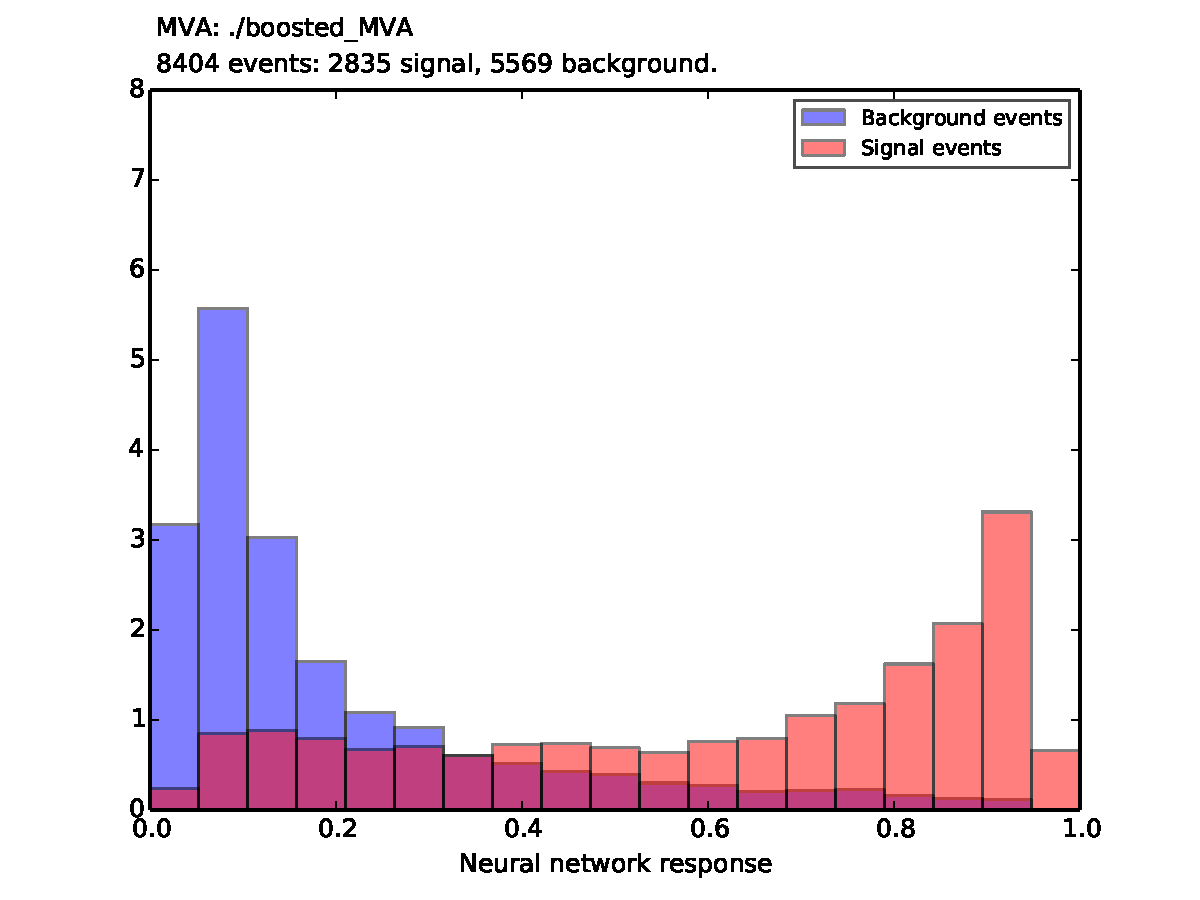
\includegraphics[width=0.48\textwidth]{plots/boosted_MVA_hist.pdf}
\caption{\small Neural network response demonstrated for the case of the resolved (left) and boosted (right) analyses. The frequency of background and signal events is plotted as a function of neural network output.
{\bf what is the y axis??}
}
\label{fig:nnresponse}
\end{center}
\end{figure}
%%%%%%%%%%%%%%%%%%%%%%%

The result of the signal selection efficiency as a function of the
background rejection rate as the value on the cut on the NN output
is varied is known as the Receiver Operating Characteristic (ROC)
curve.
%
It is clear that we can achieve a very high signal efficiency but using
a low value of the threshold, but this will have a poor background
rejection.
%
Using a higher value of the cut will increase background rejection at the
cost of dropping signal efficiency.
%
The usefulness of ROC curves is that they allow to determine the
optimal cut value that removes enough background without degrading too much the signal efficiency.

In Fig.~\ref{fig:exampleroc} the ROC curves for the
boosted, intermediate and resolved categories are found.
%
As could already be inferred from the distribution of neural
networks output in Fig.~\ref{fig:nnresponse}, we find
that the neural network MVA is reasonably efficient
in discriminating signal over background.
%
The performance is slightly better in the case of the boosted
topology, in particular thanks to the information provided
by the substructure variables.
%
In both cases we see that with a moderate reduction of signal
efficiency of $\sim 0.8$, one can reduce the background by 80\%,
which translates into an improvement factor of the pre-MVA $S/\sqrt{B}$
of almost $\sim 1.8$.



%%%%%%%%%%%%%%%%%%%%%%%%%%%%%%%%%%%%%%%%%%%%%%
\begin{figure}[t]
\begin{center}
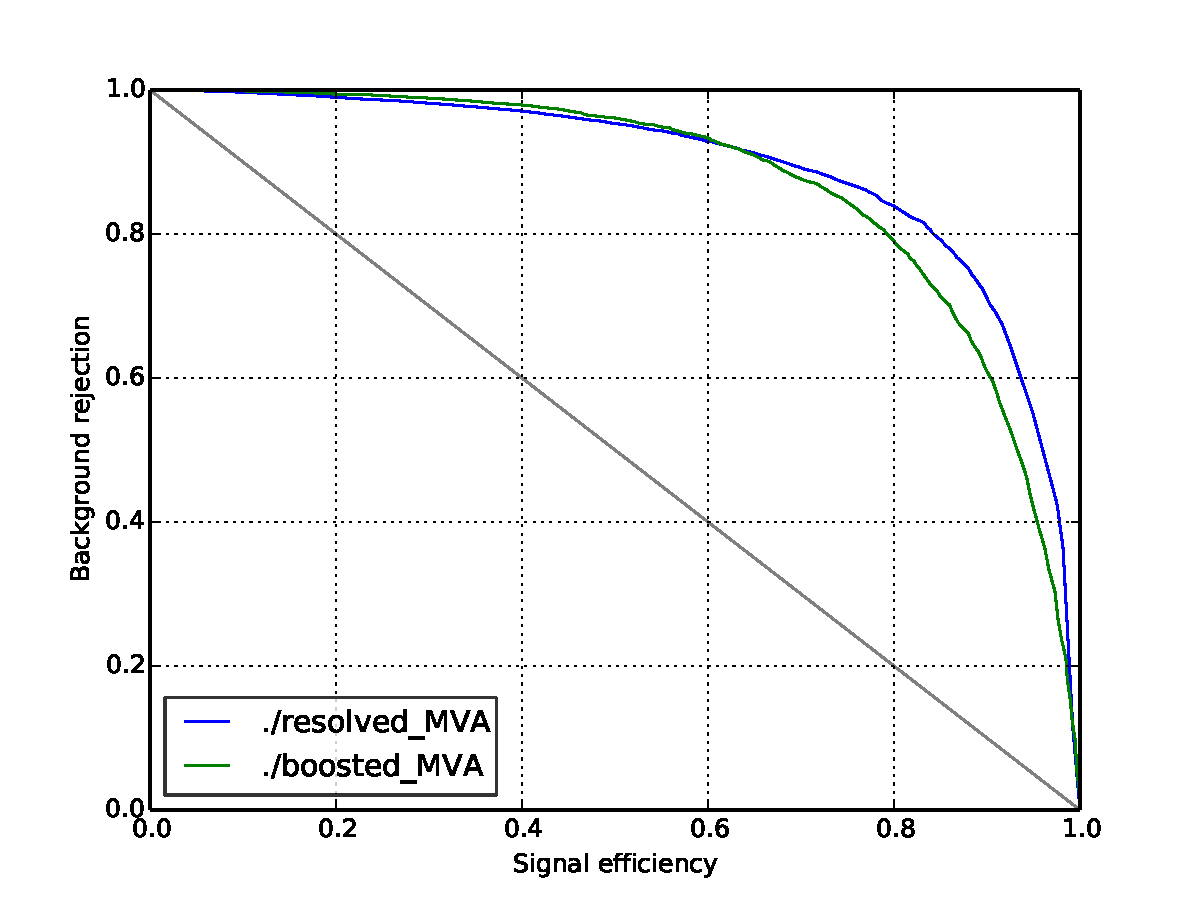
\includegraphics[width=0.65\textwidth]{plots/example_roc.pdf}
\caption{\small ROC curve for the neural network discriminant in the boosted (green) and resolved (blue) cases.}
\label{fig:exampleroc}
\end{center}
\end{figure}
%%%%%%%%%%%%%%%%%%%%%%%%%%%%%%%%%%%%%

In order to gain physical insight of which are the variables that
contribute the most to the MVA discrimination it is useful
to show the distribution of NN weights for each of the
input variables.
%
This distributions is a measure of the correlation between
each input variable and the Neural Network output: the higher
the value, the stronger the impact of this variable in
separating signal from the background.
%
In Fig.~\ref{fig:nnweights} we show
the distribution of NN weights for the resolved and boosted categories.

%%%%%%%%%%%%%%%%%%%%%%%%
\begin{figure}[t]
\begin{center}
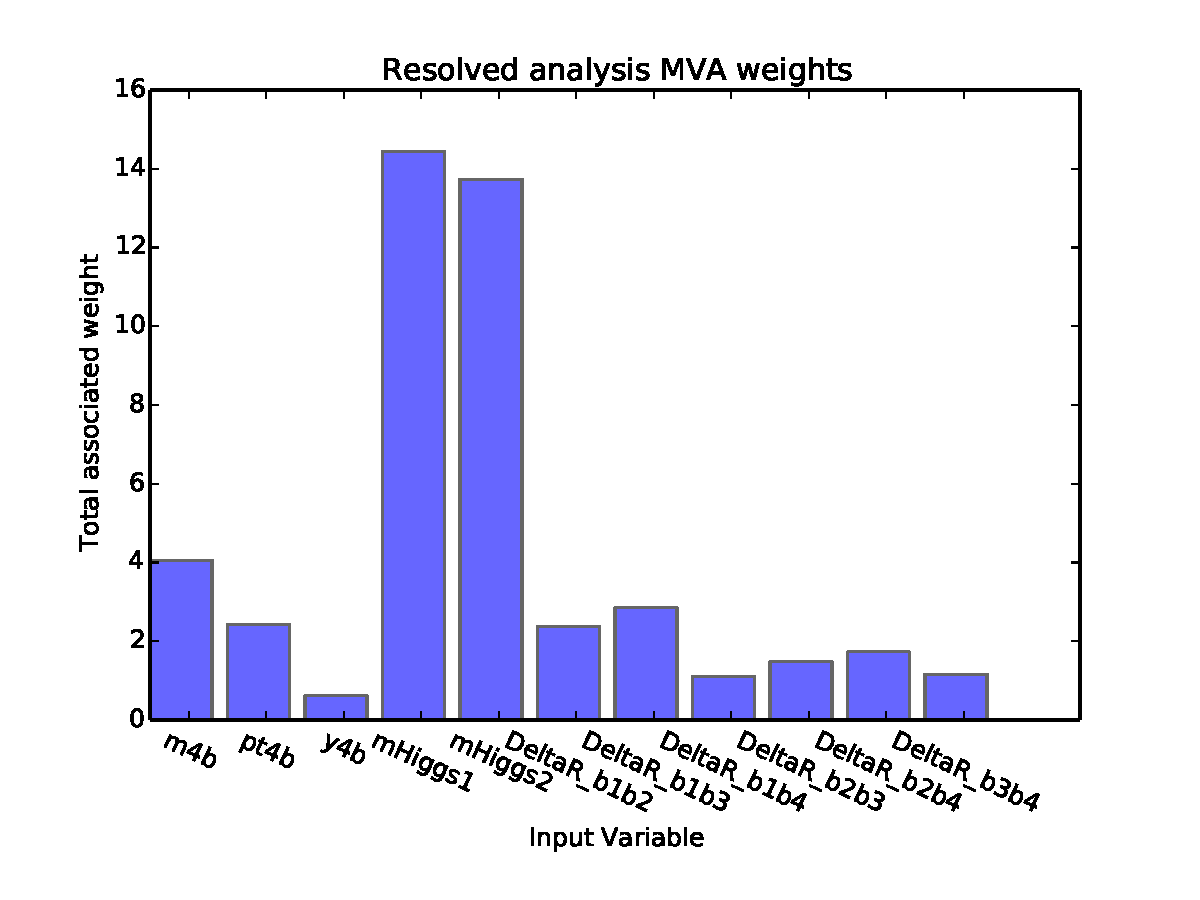
\includegraphics[width=0.48\textwidth]{plots/nnweights_res.pdf}
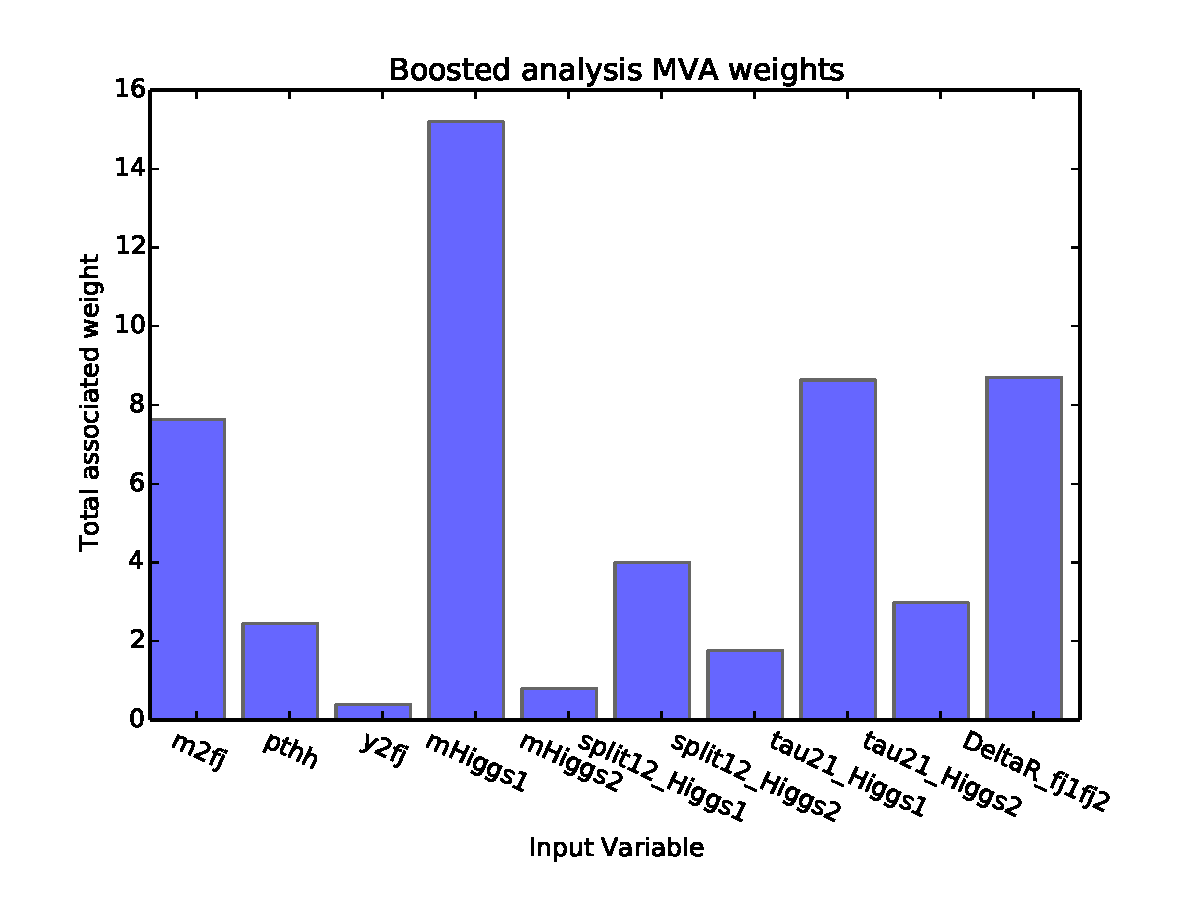
\includegraphics[width=0.48\textwidth]{plots/nnweights_boost.pdf}
\caption{\small Distribution of weights per input variable in the final ANN analysis. The above figure shows the weight distribution in the case of the resolved analysis, while the lower plot shows the boosted analysis.}
\label{fig:nnweights}
\end{center}
\end{figure}
%%%%%%%%%%%%%%%%%%%%%%%

The results of Fig.~\ref{fig:nnweights} clearly illustrate which variables
are more discriminative between the signal and the background.
%
For instance, in the case of the resolved analysis, the variables that show
a higher discrimination power is the invariant mass of the Higgs candidate dijets.
%
Note that as explained in Sect.~\ref{sec:analysis}, we have applied a realistic
smearing of the four-momentum of all reconstructed jets, but still is clear that the
distribution of invariant mass of the Higgs candidates will be very different
in the signal and in the backgrounds.
%
We discussed below the impact of smearing has.
%
Other variables do not seem to have a dramatic effect, although of course one of the
advantages of the MVA technique is that it does not hurt to add redundant
information.
%
In particular the angular distances between the four leading $b$-jets does not
provide additional information.


The corresponding analysis for the boosted category is also
shown in Fig.~\ref{fig:nnweights}.
%
Here we see that there is a more even distributions of weights, in that many
variables help in a similar amount in the discrimination.
%
The invariant mass of the Higgs candidate of course still carries a lot of weight,
but now we see that the substructure variables really carry  a lot of information,
in particular the splitting scales and the subjetiness $\tau_{12}$.
%
We have verified that signal significance in the boosted category is substantially
degraded if substructure variables are not used.






\subsection{Impact of smearing in the MVA discrimination}

Accounting for a suitable smearing of the final-state momenta of the reconstructed
jets is essential to be able to draw any realistic conclusions in analysis like
this one that are based on a large number of jets.
%
It is therefore interesting how the MVA discrimination changes if one did not account
for smearing - of course in this case differences between signal and background distributions
would be enhanced.

To investigate this, we now consider a variant of the analysis used in
Table~\ref{tab:resCutflow} where the $m_H$ window criterion has been relaxed to $80 < m_H < 170$.
%
Firstly the same analysis is repeated with the larger $m_H$ window, with no smearing at all.
%
This is then compared to the same analysis but with a Gaussian smearing with $\sigma=10$ GeV applied to the dijet invariant mass used in the MVA.
%
In the left panel of Fig.~\ref{fig:invMsmear} the smearing is demonstrated.
%
Both with and without smearing, the  invariant mass distribution of the
Higgs candidates is still the most discriminative variable.
%
This can be seen by comparing with   with the corresponding distribution with smearing in
  Fig.~\ref{fig:nnweights}.




%%%%%%%%%%%%%%%%
\begin{figure}[t]
\begin{center}
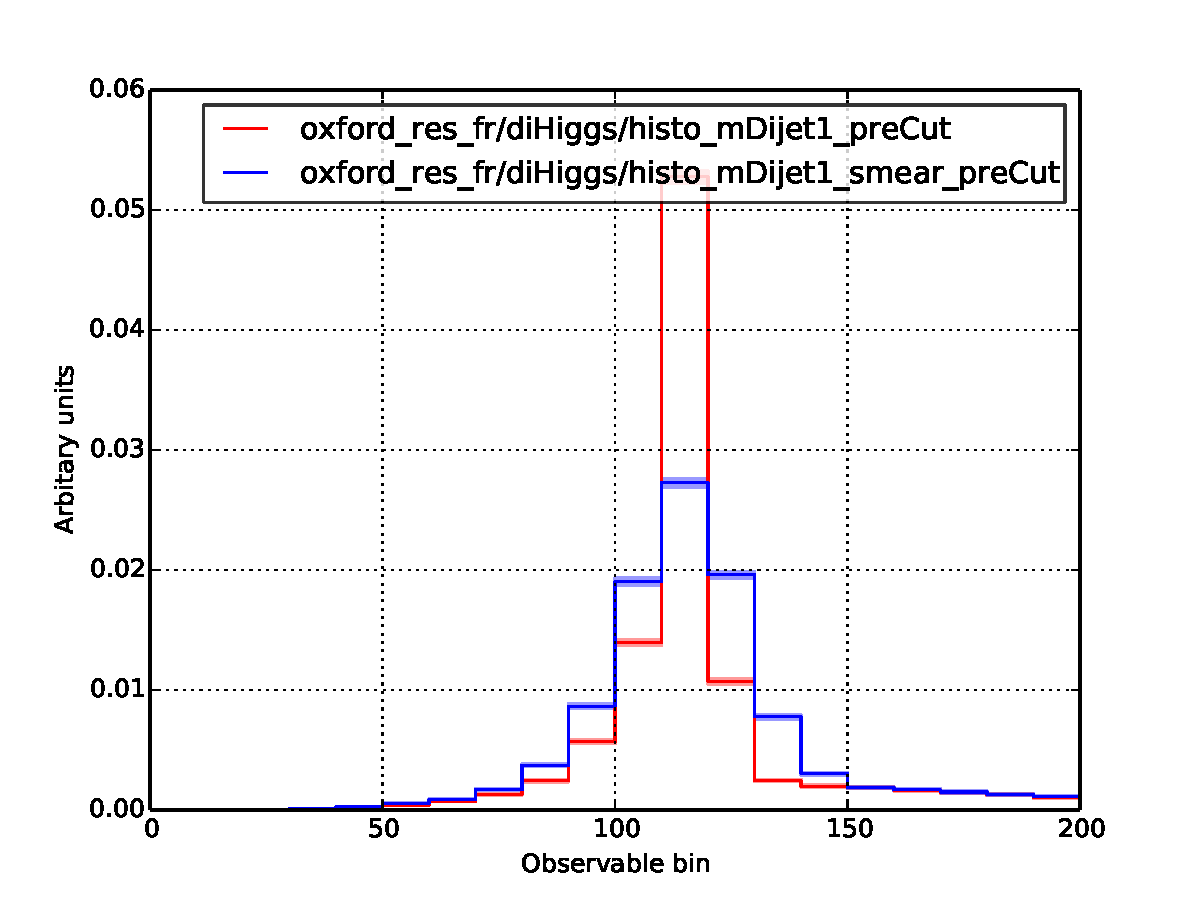
\includegraphics[width=0.49\textwidth]{plots/Msmear/histo_mass_smear_precut.pdf}
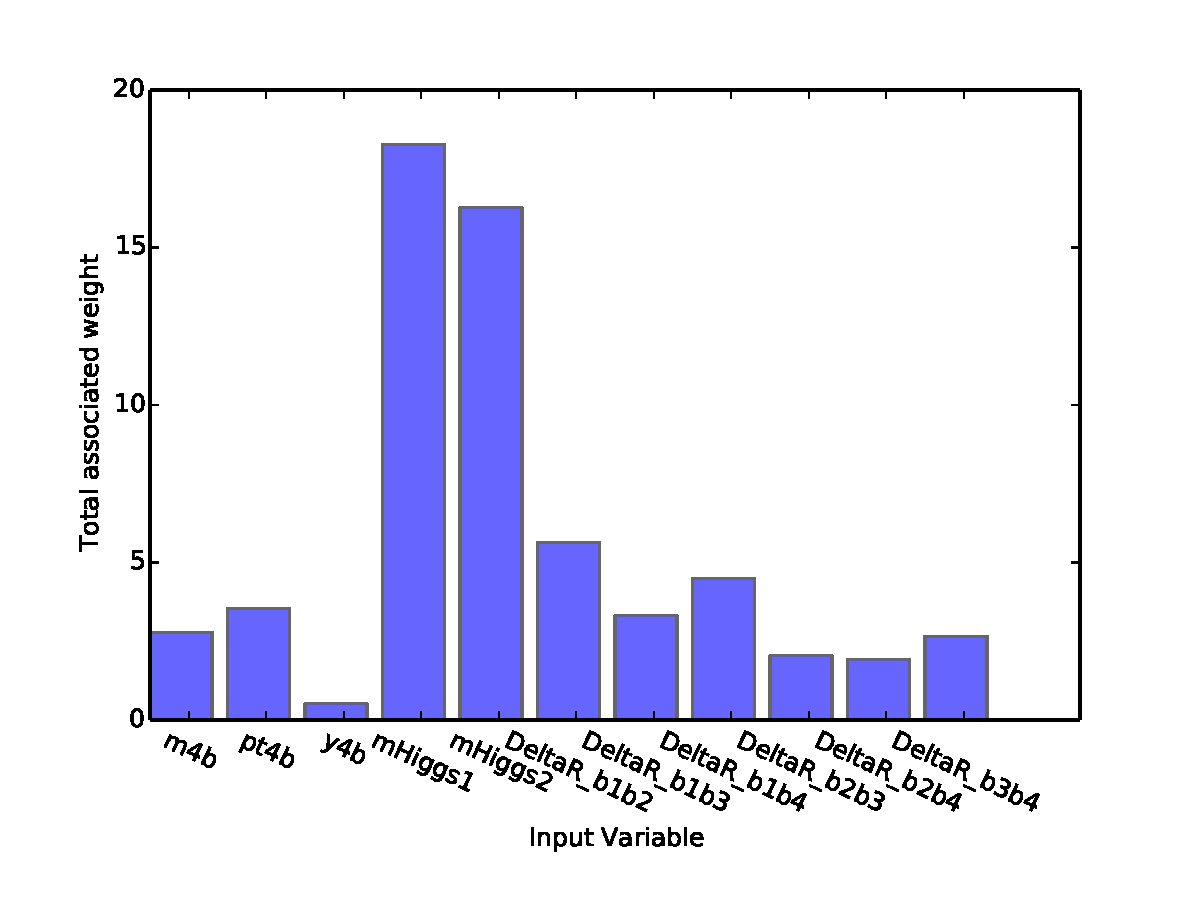
\includegraphics[width=0.49\textwidth]{plots/Msmear/nnweights.pdf}
\caption{\small Left plot: the invariant mass distribution of the
  Higgs candidates without (red) and with (blue) smearing.
  %
  Right plot: the strength of the NN weights in the resolved case when no smearing
  is applied.
  %
  It should be compared with the corresponding distribution with smearing in
  Fig.~\ref{fig:nnweights}.
  %
  As expected, the discrimination power of the invariant mass distribution is
  enhanced if there is no smearing.}
\label{fig:invMsmear}
\end{center}
\end{figure}
%%%%%%%%%%%%%%%%%
  

While the MVA still derives most of it's discriminating power from the dijet masses, the smearing reduces it's effectiveness considerably.
%
In Fig.~\ref{fig:smearedROC} the ROC curves of the MVA applied to the smeared and unsmeared distributions are shown, where it is clear that the overall performance of the MVA is significantly hampered by the smeared invariant masses.
%
For example, if we require the same signal efficiency as before, 0.8, the background rejection
is degraded from 80\% down to 60\%.
%
Therefore, we can conclude that it is important to include smearing to draw realistic
conclusions, though the qualitative information of which are the most relevant
discriminative variables is not changed by this conclusion.


%%%%%%%%%%%%%%%%%
\begin{figure}[t]
\begin{center}
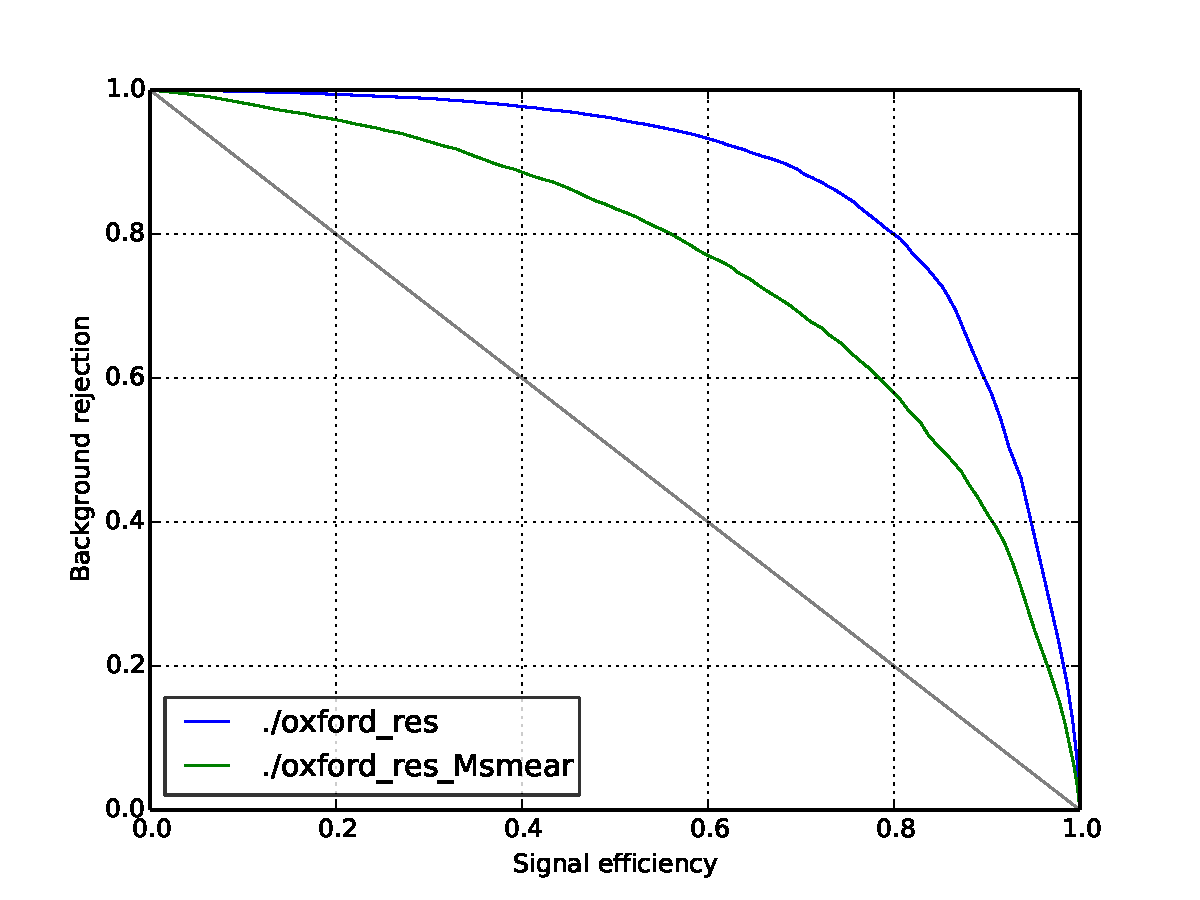
\includegraphics[width=0.50\textwidth]{plots/Msmear/roc.pdf}
\caption{\small ROC curves of the MVA applied with the unsmeared (blue) and smeared (green) dijet invariant mass distributions.}
\label{fig:smearedROC}
\end{center}
\end{figure}
%%%%%%%%%%%%%%%%
            
